\section{G-set の 9 問題での検証}\label{sec:gset}

\subsection{設定}

事前登録の結果（\ref{sec:prereg} 節）と小規模問題の結果（\ref{sec:small} 節）を受けて，判定基準を実行前に固定した計画をコミットしてから，G-set の 9 問題で C1・C2 を調べた．問題は，ランダムグラフ G1（800 頂点），G22，G23（2000），G55（5000），G70（10000），平面グラフ G14，G15（800），G39（2000），トーラス G32（2000）である．重みは G32 と G39 が $\pm1$，ほかは 1 である．計画には G77（トーラス，14000 頂点）も含めていたが，計算時間の都合で，結果を見る前に除いた．

CIM は 2400 ラウンド（全問題で収束を確認）とし，事前登録の実行と重ならない seed で各問題 $K=512$ 個の候補を作った．SA は開始温度 $T_0=0.5$ と $2.0$，予算 50・500・5000 掃引で，各候補に $R=16$ 回かけた．試し打ちは 50 掃引の SA を 2 回とした．問題 × 温度 × 予算の 54 条件で，C1（残差の split-half 信頼性）と指標ごとの $\rho$ を求めた．

固定した判定は次の 4 つである．
\begin{description}
  \item[H3a] CIM の出力が多様な問題（異なる状態が候補の半分以上）では，$T_0=0.5$ のいずれかの予算で C1 が成り立つ．
  \item[H3b] $T_0=2.0$・5000 掃引で C1 が成り立つ問題では，$\rho(E,r)$ の区間の下限が 0 を超える（主検定 R1 の一般化）．
  \item[H3c] C1 が成り立つ条件では，試し打ちの $\rho$ の区間の下限が 0 を超える．
  \item[H3d] C1 が成り立つ条件では，LS 後に利得が $-2$〜$0$ の頂点数の $\rho$ の区間の上限が 0 を下回る（小規模問題での向き）．
\end{description}

\paragraph{解析後の変更.} 事前登録と同じく，SA が種を超えずラベルが初期カット値と一致する条件は判定不能とする計画だった．しかし判定に使っていた「残差の幅 $<10^{-9}$」は，カット値が $10^4$ 程度の問題では最小二乗の丸め誤差で通り抜け，G55（$T_0=2.0$・50 掃引）で見かけの C1 $=1.00$ が出た．また G70（$T_0=2.0$・50・500 掃引）では，512 候補のうち 1 候補だけが種を超え，相関がその 1 候補で決まっていた．そこで「SA が種を一度でも超えた候補が 5\% 未満なら判定不能」に改め，この 3 条件を判定不能とした．ほかの 51 条件の値は変わらない．

\subsection{結果}

図\ref{fig:gset}に全条件の結果を示す．C1 が成り立ったのは 54 条件中 33 条件だった．

\begin{figure}[t]
\centering
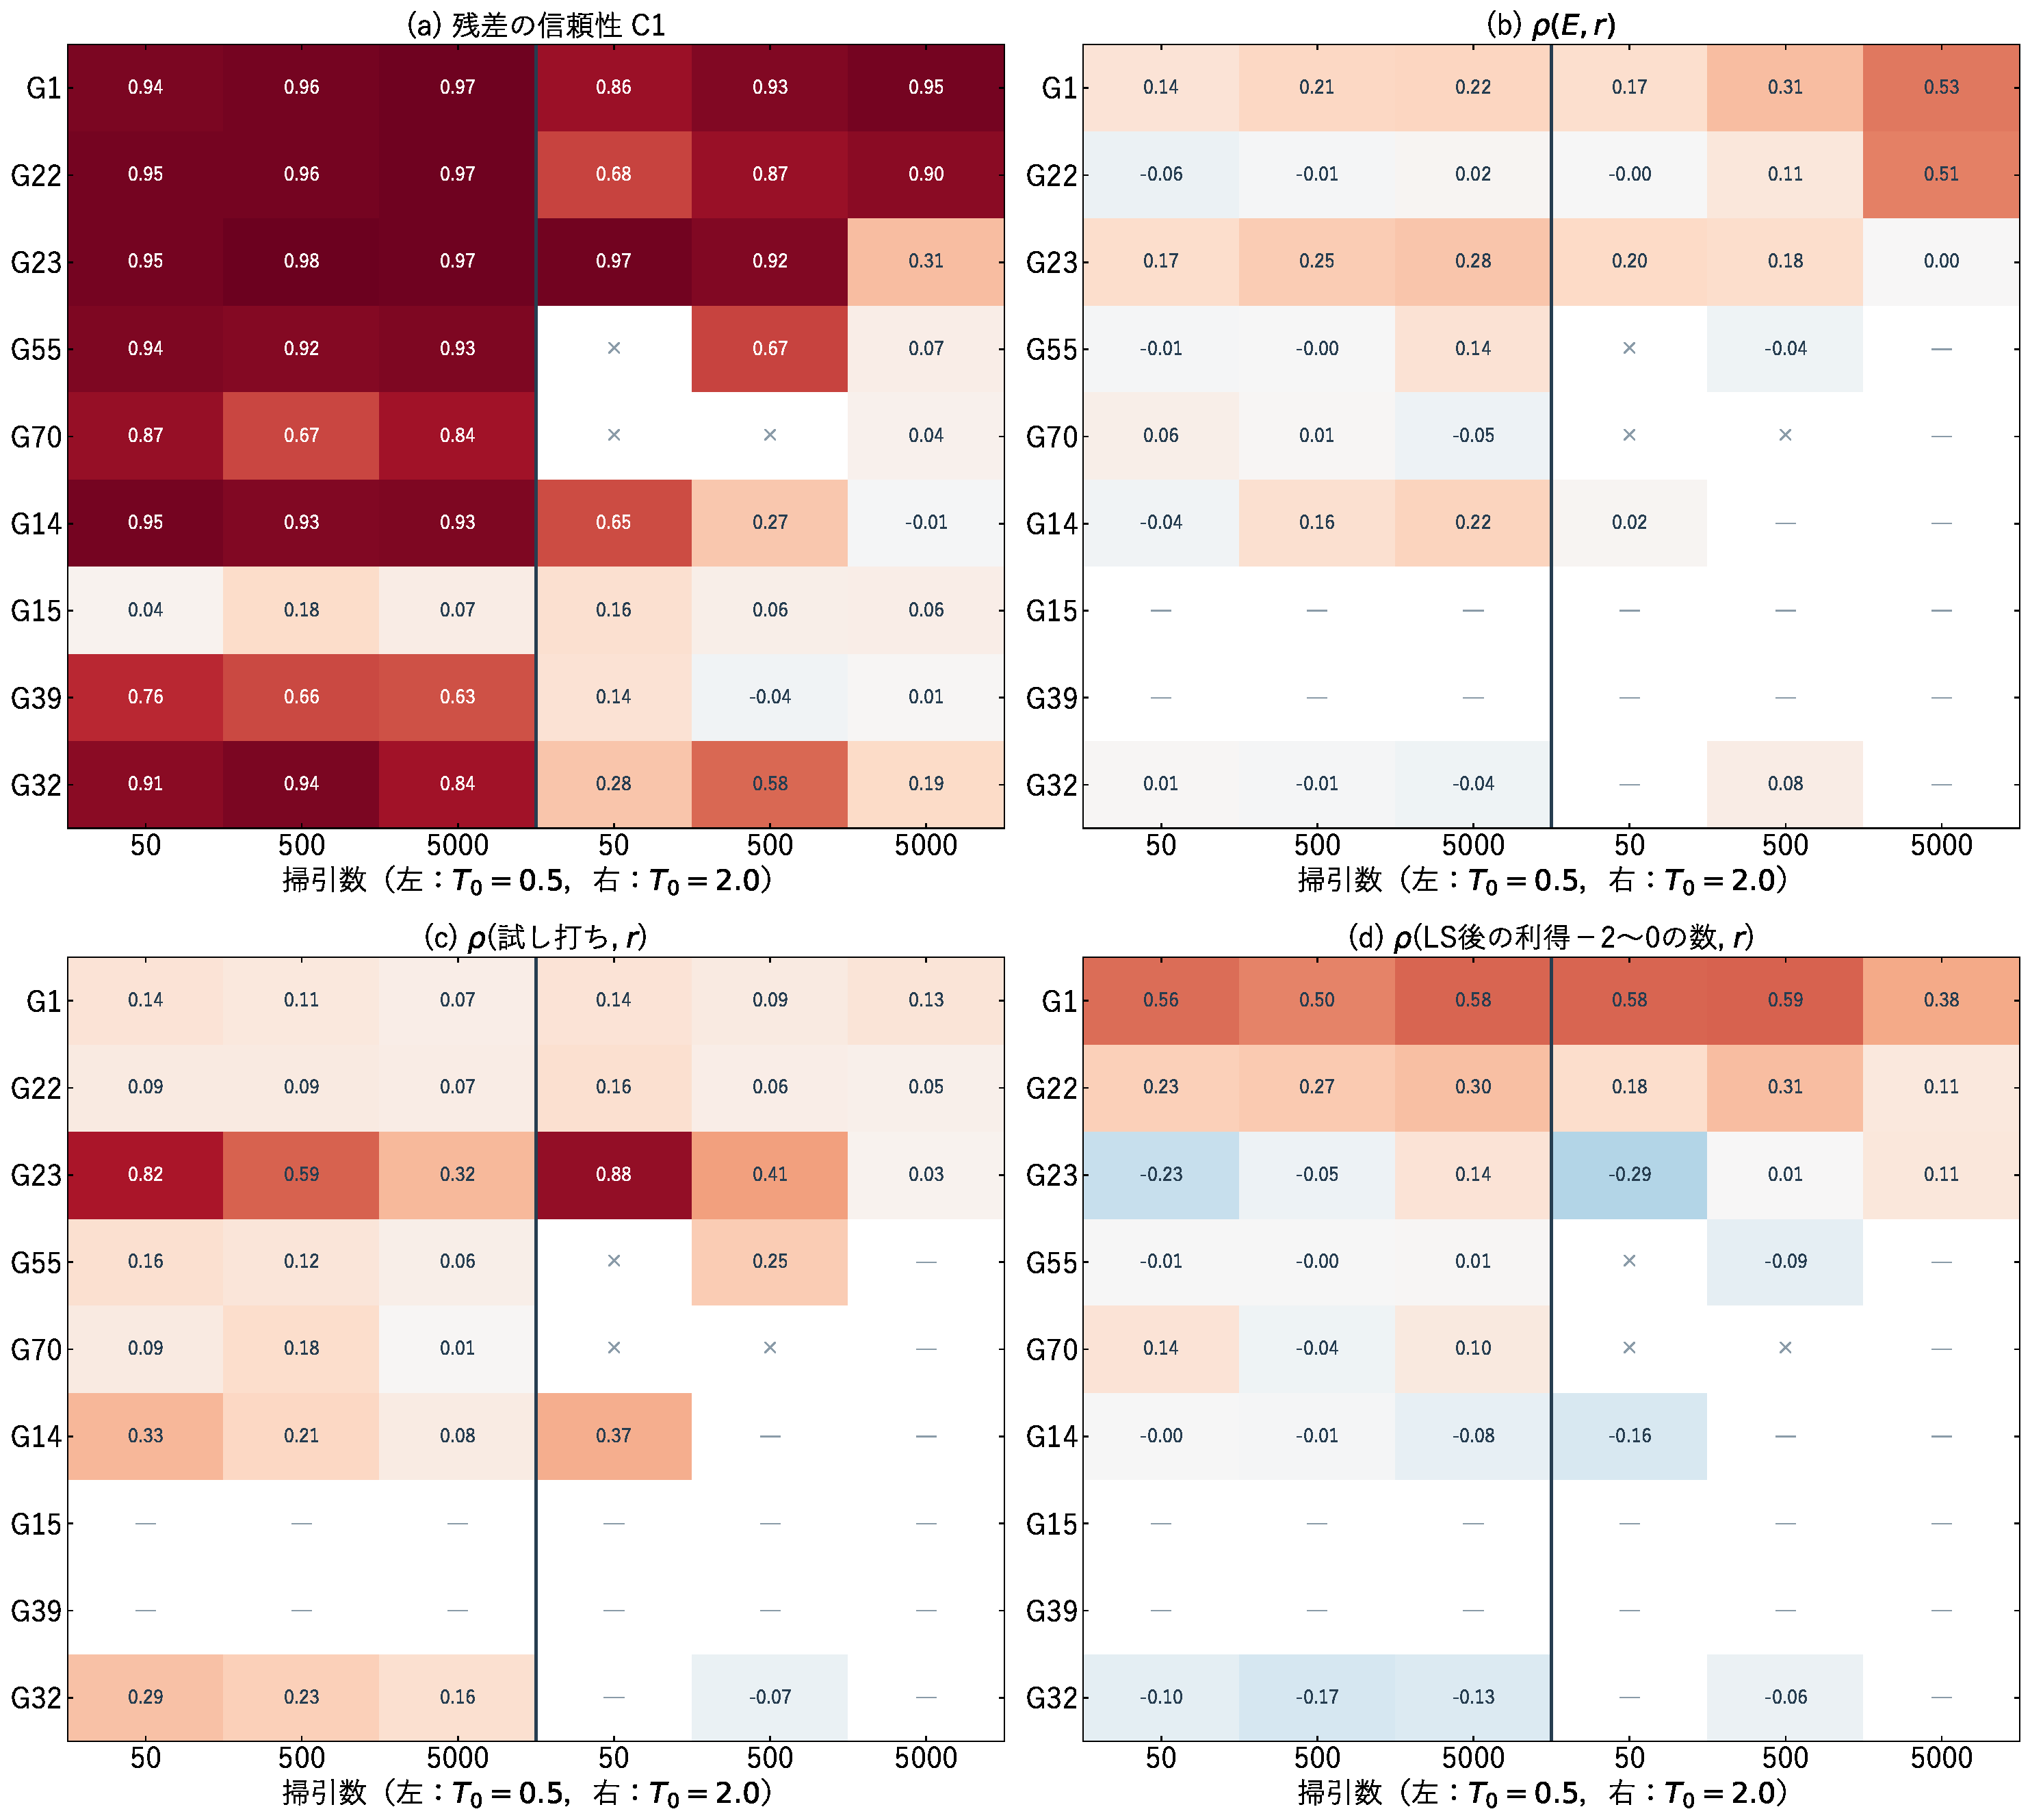
\includegraphics[width=\linewidth]{fig_gset.pdf}
\caption{G-set の 9 問題の結果．各マスは問題 × 開始温度 × 予算．(a) 残差の split-half 信頼性．(b)〜(d) 指標と残差の Spearman $\rho$（C1 が成り立った条件だけ色をつけた）．「×」は判定不能（SA が種をほとんど超えない），「—」は C1 が成り立たない条件．}\label{fig:gset}
\end{figure}

\paragraph{C1 は CIM の出力が多様なら成り立つ（H3a 成立）.} 出力が多様な 7 問題（異なる状態 303〜512 個）のすべてで，$T_0=0.5$ の 3 つの予算すべてで C1 が成り立った（信頼性 0.67〜0.98）．$T_0=0.5$ の SA は種の近くを探すので，カット値と LS で説明できない候補ごとの差がはっきり残る．$T_0=2.0$ では予算が長いほど信頼性が下がり，5000 掃引で C1 が残ったのは G1（0.95），G22（0.90），G23（0.31）だけだった．これは事前登録の実行で見た「SA が種を忘れると差が消える」という傾向（\ref{sec:prereg} 節）と同じである．平面グラフの G15 と G39 では，CIM の出力が 1 個と 5 個の状態に集まり，選別の余地がそもそもなかった．

\paragraph{固有ベクトル指標は G1 と G22 で効く（H3b 一部成立）.} $T_0=2.0$・5000 掃引で C1 が成り立った 3 問題のうち，$E$ は G22（$\rho=0.51$，[$0.43$, $0.57$]）と G1（$0.53$，[$0.46$, $0.60$]）で効き，G23（$0.00$，[$-0.09$, $0.09$]）では効かなかった．G22 では新しい seed で 3 回目の再現であり，G1 という別の問題でも同じ大きさで成り立った．どちらも重み 1 のランダムグラフで，$E$ が効くのは長い予算のときだけという点も共通している（G1 の $\rho$ は 50・500・5000 掃引で 0.17，0.31，0.53）．一方，G23 は G22 と同じ種類のグラフだが，長い予算では効かず，$T_0=0.5$ で弱く効いた（0.17〜0.28）．C1 が成り立つ 33 条件のうち，$E$ の区間が正だったのは 16 条件である．

\paragraph{試し打ちは広く効くが弱い（H3c 成立）.} 試し打ちは 33 条件中 28 条件で区間の下限が 0 を超えた．ただし多くの問題で $\rho=0.05$〜$0.3$ と小さい．G23 の短い予算だけは $0.6$〜$0.9$ と強かった．

\paragraph{局所的な指標の向きは問題で逆転する（H3d 不成立）.} LS 後に利得が $-2$〜$0$ の頂点数は，小規模問題では価値と負の相関を持っていたが，G-set では予想の向きだったのは 33 条件中 6 条件（G32 と G14，G55 の一部）だけだった．G1 と G22 ではむしろ正の相関（$\rho=0.1$〜$0.6$）を持った．向きを予想しなかった $g_i=0$ の頂点数は 33 条件中 24 条件で区間が 0 を除いたが，その向きも問題によって違った．

以上から，C1 は多様な出力を持つすべての問題で成り立つ頑健な現象である一方，C2 の答えは問題に依存する．問題をまたいで同じ向きに効いたのは試し打ちだけであり，固有ベクトル指標は重み 1 のランダムグラフの長い予算という特定の状況で強く効く．
